\section{Quantenalgorithmen}
\subsection{Der Umstieg von derzeitigen Digitalen Signaturen zu PQC}
Die heutigen Digitalen Signaturen ((EC)DSA, (EC)ElGamal) basieren auf dem diskreten Logarithmus Problem oder bei RSA auf der schwierigkeit des faktorisierens großer Semi-Primzahlen in dessen Primfaktoren.
RSA hat den Vorteil, dass die verschlüsselung und die Signatur sich nicht stark von einander unterscheiden.\cite{paarKryptografieVerstaendlichLehrbuch2016}

Die Verfahren aus dem NIST-Auswahlprozess haben längere Signaturen und nicht so einfach wie RSA.
Der Signatur- und Verschlüsselungsalgorithmus unterscheiden sich stärker voneinander. Für DNSSEC sind nur die Signaturen interessant.

\subsubsection{Crystals-Dilithium}
Das von der NIST favorisierte Verfahren, es wurde unter anderem von Deutschen Kryptographen entwickelt und basiert auf der schwierigkeit den nächsten Gitterpunkt zu einem Punkt in einem Hochdimensionalem Gitter zu finden.
Es wird ein Gleichungssystem aufgestellt für das eine Lösung mit kleinen Zahlen gefunden werden muss.
Es basiert auf dem Short Integer Solution (SIS) Problem.
Das Gleichungssystem, welches auch der öffentliche Schlüssel ist, enthält zudem kleine Fehler.
Der private Schlüssel ist die Lösung dieses Gleichungssystems.
Um aus der Einwegfunktion (aufstellen eines fehlerhaftes Gleichungssystems) ein valides Kryptosystem zu bauen, wird die sog. Fiat-Shamir Funktion angewandt.
Wenn die Einwegfunktion sich auch mit Quantencomputern nicht effizient lösen lässt, ist das Verfahren durch die Fiat-Shamir-Transformation Quanten sicher.\cite{schmehFiatShamirTransformation2026,schmehGitterbasierteAlgorithmen2026}

\begin{figure}[htbp]
    \centering
    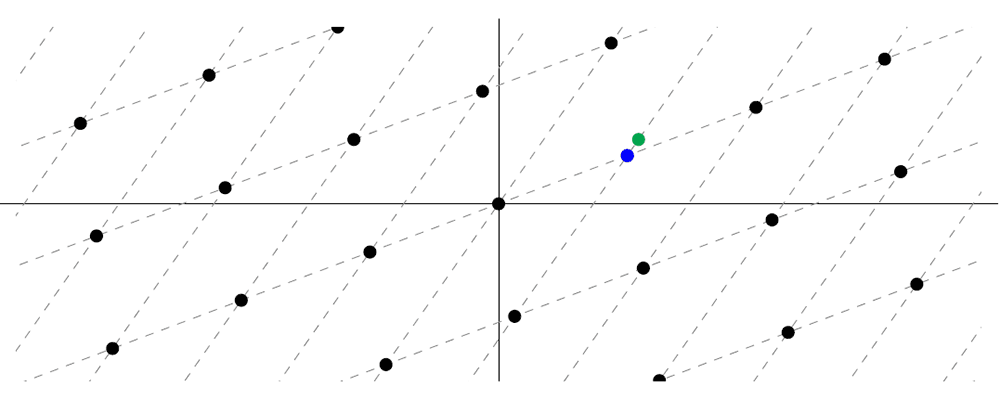
\includegraphics[width=1.0\textwidth]{bilder/gitter-sis}
    \caption{2-dimensionales Gitter mit einem Punkt und dem nächstgelegenen Gitterpunkt. Quelle: \url{https://1000children.org/lattice-cryptography-example-overview-of-lattice-based-cryptography/}}\hfill
    \label{fig:gitter-sis}
\end{figure}

Abbildung \ref{fig:gitter-sis} zeigt das SIS-Problem in einem zweidimensionalen Gitter.
Von dem grünen Punkt aus soll der nächstgelegene Gitterpunkt (in blau dargestellt) gefunden werden.
Es muss ein höherdimensionales Gitter und eine schlechte Basis verwendet werden, damit das Problem schwer genug ist\cite{schmehGitterbasierteAlgorithmen2026}.

\subsubsection{FALCON}
\textbf{Fa}st-Fourier \textbf{L}attice-based \textbf{Co}mpact Signatures over \textbf{N}TRU, kurz FALCON.
Das einzige dieser Kryptosystem, welches mit Gleitkommzahlen rechnet.
Es basiert auch auf dem Short Integer Solution (SIS) Problem über NTRU Gittern.
FALCON gilt aufgrund von Gleitkommazahlen, rekursiven Funktionen und mehreren diskreten Gaussverteilungen als schwerig zu implementieren.
FALCON hat den Vorteil, dass es kleine Signaturen und öffentliche Schlüssel hat und das es schneller im verifizieren ist.
Unter anderem nutzt es die Fast-Fourier-Transformation mit einer Superlinearen Laufzeitkomplexität von $O(n \log n)$ anstelle der Fourier-Transformation mit einer quadratischen Laufzeitkomplexität $O(n^2)$.\cite{nguyenFastFalconSignature2023,soniFALCON2021}
Crystals-Dilithium und FALCON nutzen zur Verifikation \enquote{Fiat-Shamir with aborts}, welches ein challenge-response Verfahren ist\cite{LatticeSignaturesFiatShamir}.

\subsubsection{Rainbow}
Rainbow ist ein multivariates Polynomiales Kryptosystem, welches eine Generalisierung des Oil and Vinegar scheme (UOV) ist.
Das unterliegende Problem ist, dass ein multivariates Gleichungssystem von Polynomen über einem endlichen Feld ein NP-schweres Problem ist.
Ein Gleichungssystem wie das folgende (aus serious cryptography\cite{aumassonSeriousCryptographyPractical2018}) mit vier unbekannten ist gegeben, um es zu lösen müssen alle vier unbekannten $x_1,x_2,x_3,x_4$ gefunden werden.
\begin{align*}
&x_1x_2\ +\ x_3x_4\ +\ x_2\ =\ 1\\
&x_1x_3\ +\ x_1x_4\ +\ x_2x_3\ =\ 12\\
&x_{1}^2\ +\ x_{3}^2\ +\ x_4\ =\ 4\\
&x_2x_3\ +\ x_2x_4\ +\ x_1\ x_4\ =\ 0
\end{align*}
Solch ein Gleichungssystem zu lösen ist NP-schwer und lässt sich auch mit Quantencomputern nicht effizient lösen.
Multivariate Kryptosysteme wurden bereits öfters gebrochen, trotz der Annahme sicher zu sein und die Berechnungen sich oft auch ressourcen lastig, auch wenn die Signaturen eher kurz sind, was dazu führt, dass der Einsatz dieser Systeme in der Praxis recht selten ist\cite{aumassonSeriousCryptographyPractical2018}.
Das Rainbow kryptosystem wird beschrieben als eine mehrschichtige oil-and-vinegar konstruktion und dessen generalisierung\cite{dingRainbowNewMultivariable2005}.

\subsubsection{weitere PQC-Signatur-Verfahren}
\textbf{Hash-basierte} Signaturen bauen auf der Sicherheit von Hash-Funktionen auf.